%!TEX program=xelatex

% 碰到Windows版本提示Fandol字体,可以在命令行中以管理员权限执行:tlmgr update -self -all
%\documentclass[review]{cvpr}
\documentclass[final]{cvpr}

\usepackage[UTF8]{ctex}

%\usepackage{cvpr}
\usepackage{times}
\usepackage{epsfig}
\usepackage{graphicx}
\usepackage{amsmath}
\usepackage{amssymb}
\usepackage{subfigure}
\usepackage{overpic}
\setlength{\parindent}{2em}
\usepackage{enumitem}
\usepackage{indentfirst}
\setenumerate[1]{itemsep=0pt,partopsep=0pt,parsep=\parskip,topsep=5pt}
\setitemize[1]{itemsep=0pt,partopsep=0pt,parsep=\parskip,topsep=5pt}
\setdescription{itemsep=0pt,partopsep=0pt,parsep=\parskip,topsep=5pt}


\usepackage[pagebackref=true,breaklinks=true,colorlinks,bookmarks=false]{hyperref}


%\cvprfinalcopy % *** Uncomment this line for the final submission

\def\cvprPaperID{159} % *** Enter the CVPR Paper ID here
\def\confYear{CVPR 2020}
\def\httilde{\mbox{\tt\raisebox{-.5ex}{\symbol{126}}}}

\newcommand{\cmm}[1]{\textcolor[rgb]{0,0.6,0}{CMM: #1}}
\newcommand{\todo}[1]{{\textcolor{red}{\bf [#1]}}}
\newcommand{\alert}[1]{\textcolor[rgb]{.6,0,0}{#1}}

\newcommand{\IT}{IT\cite{98pami/Itti}}
\newcommand{\MZ}{MZ\cite{03ACMMM/Ma_Contrast-based}}
\newcommand{\GB}{GB\cite{conf/nips/HarelKP06}}
\newcommand{\SR}{SR\cite{07cvpr/hou_SpectralResidual}}
\newcommand{\FT}{FT\cite{09cvpr/Achanta_FTSaliency}}
\newcommand{\CA}{CA\cite{10cvpr/goferman_context}}
\newcommand{\LC}{LC\cite{06acmmm/ZhaiS_spatiotemporal}}
\newcommand{\AC}{AC\cite{08cvs/achanta_salient}}
\newcommand{\HC}{HC-maps }
\newcommand{\RC}{RC-maps }
\newcommand{\Lab}{$L^*a^*b^*$}
\newcommand{\mypara}[1]{\paragraph{#1.}}

\graphicspath{{figures/}}

% Pages are numbered in submission mode, and unnumbered in camera-ready
%\ifcvprfinal\pagestyle{empty}\fi
\setcounter{page}{409}
\begin{document}
% \begin{CJK*}{GBK}{song}

\renewcommand{\figref}[1]{图\ref{#1}}
\renewcommand{\tabref}[1]{表\ref{#1}}
\renewcommand{\equref}[1]{式\ref{#1}}
\renewcommand{\secref}[1]{第\ref{#1}节}
\def\abstract{\centerline{\large\bf 摘要} \vspace*{12pt} \it}

%%%%%%%%% TITLE

\title{基于欧拉方法的一维热传导数值求解问题}

\author{任立德\\
    南方科技大学\\
}

\maketitle
% \thispagestyle{empty}

%%%%%%%%% ABSTRACT
\begin{abstract}
	\setlength{\parindent}{2em}
本项目完成了对一维热传导方程的数值求解。在时间上采用了显式欧拉方法和隐式欧拉方法,在空间上采用了有限差分方法。通过调用PETSC完成对向量和矩阵对运算,通过调用MPI实现并行计算,通过HDF5文件保存数据。通过调整网格点大小和时间步大小对两种方法对稳定性和误差进行了分析。通过使用“-r”参数控制程序是否重启。通过使用“-np”调整CPU核数对代码并行效率进行分析。
\end{abstract}




%%%%%%%%% BODY TEXT %%%%%%%%%%%%%%%%%%%%%%%%%%%%%%%%%%%%%%%%
\section{理论推导}\label{sec:Introduction}
\setlength{\parindent}{2em}
已知一维热传导方程如下所示。
\begin{center}
		\begin{scriptsize}
\begin{equation}
	\setlength{\abovedisplayskip}{-5pt}
\rho c \frac{\partial u}{\partial t}-\kappa \frac{\partial^{2} u}{\partial x^{2}}=f
\end{equation}
\end{scriptsize}
\end{center}

根据有限差分法和显式欧拉方法可以得到如下公式。
\begin{center}
		\begin{scriptsize}
	\begin{equation}
			\setlength{\abovedisplayskip}{-5pt}
				\rho c \frac{u_{j}^{n+1}-u_{j}^{n}}{\Delta t}-\kappa \frac{u_{j-1}^{n}-2 u_{j}^{n}+u_{j+1}^{n}}{\Delta x^{2}}=f
	\end{equation}
\end{scriptsize}
\end{center}

经过推导得到第n+1个时间步,第j个网格点的$u_{j}^{n+1}$计算公式。
\begin{center}
	\begin{scriptsize}
	\begin{equation}
		\setlength{\abovedisplayskip}{-5pt}
		u_{i}^{n+1}=\frac{\kappa \Delta t}{\rho c \Delta x^{2}} u_{j-1}^{n}+\left(1-\frac{2\kappa \Delta t}{\rho c \Delta x^{2}}\right) u_{j}^{n} +\frac{\kappa \Delta t}{\rho c \Delta x^{2}} u_{j+1}^{n}+\frac{f \Delta t}{\rho c}
	\end{equation}
\end{scriptsize}
\end{center}

定义$\alpha=\frac{\kappa \Delta t}{\rho c \Delta x^{2}}$,则问题可以转换成三对角矩阵的求解。
\begin{center}
	\begin{scriptsize}
		\begin{equation}
			\setlength{\arraycolsep}{1pt}
			\setlength{\abovedisplayskip}{-5pt}
\left[\begin{array}{cccc}
	1-2 \alpha & \alpha& &  \\
	\alpha & 1-2\alpha & \alpha&  \\
	& \ddots & \ddots &  \\
	& &  \alpha& 1-2\alpha
\end{array}\right] \times\left[\begin{array}{c}
	u_{0}^{n} \\
	u_{1}^{n} \\
	\vdots \\
	u_{j}^{n}
\end{array}\right]+\left[\begin{array}{c}
	f_{0} \\
	f_{1} \\
	\vdots \\
	f_{j}
\end{array}\right]=\left[\begin{array}{c}
	u_{0}^{n+1} \\
	u_{1}^{n+1} \\
	\vdots \\
	u_{j}^{n+1}
\end{array}\right]
		\end{equation}
	\end{scriptsize}
\end{center}

同理根据有限差分法和隐式欧拉方法可以得到推导公式。
\begin{center}
	\begin{scriptsize}
		\begin{equation}
			\setlength{\abovedisplayskip}{-5pt}
-\frac{\kappa \Delta t}{\rho c \Delta x^{2}} u_{j-1}^{n+1}+\left(1+\frac{2\kappa \Delta t}{\rho c \Delta x^{2}}\right) u_{j}^{n+1}-\frac{\kappa \Delta t}{\rho c \Delta x^{2}} u_{j+1}^{n+1}=u_{j}^{n}+\frac{f \Delta t}{\rho c}
		\end{equation}
	\end{scriptsize}
\end{center}

隐式欧拉方法同样可以转换成三对角矩阵进行求解。
\begin{center}
	\begin{scriptsize}
		\begin{equation}
			\setlength{\arraycolsep}{1pt}
			\setlength{\abovedisplayskip}{-5pt}
\left[\begin{array}{cccc}
	1+2 \alpha & -\alpha & &  \\
	-\alpha & 1+2 \alpha & -\alpha &  \\
	& \ddots & \ddots & \\
	&  & -\alpha & 1+2\alpha
\end{array}\right] \times\left[\begin{array}{c}
	u_{0}^{n+1} \\
	u_{1}^{n+1} \\
	\vdots \\
	u_{j}^{n+1}
\end{array}\right]=\left[\begin{array}{c}
	u_{0}^{n} \\
	u_{1}^{n} \\
	\vdots \\
	u_{j}^{n}
\end{array}\right]+\left[\begin{array}{c}
	f_{0} \\
	f_{1} \\
	\vdots \\
	f_{j}
\end{array}\right]
		\end{equation}
	\end{scriptsize}
\end{center}

为了验证计算过程是否正确,还需要精确解作为参考。当$\frac{\partial u}{\partial t}=0$时,系统温度不随时间变化,可以看作稳定状态。即有如下公式。
\begin{center}
	\begin{scriptsize}
		\begin{equation}
			\setlength{\abovedisplayskip}{-5pt}
-\kappa \frac{\partial^{2} u}{\partial x^{2}}=\sin (l \pi x)
		\end{equation}
	\end{scriptsize}
\end{center}

根据边界条件求得微分方程的解析解为如下公式。
\begin{center}
	\begin{scriptsize}
		\begin{equation}
			\setlength{\abovedisplayskip}{-5pt}
			u(x)=\frac{1}{\kappa l^{2} \pi^{2}} \sin (l \pi x)
		\end{equation}
	\end{scriptsize}
\end{center}
%%%%%%%%%%%%%%%%%%%%%%%%%%%%%%%%%%%%%%%%%%%%%%%%%%%%%%%%%%%%%%%%%%%%%%%%%%%%%%%%%
\section{代码实现}
\label{sec:RelatedWorks}
项目将代码分成多个模块,每个模块解决特定问题。显式方法和隐式方法除了矩阵运算模块内部实现有所差别,其他模块基本相同。

在explicit.c中,模块一定义了与模型有关的多个常量参数,包括方程中的Rho、C、K等物理量以及GRID、TSTEP等控制网格点和迭代步长的参数。模块二定义了所需变量,包括计算时所需的向量和矩阵以及并行所需的rank变量和文件变量等。模块三对参数进行初始化,包括初始化petsc和mpi,以及读取“-r”参数。模块四计算并打印模型运算的重要信息,包括dx、dt等。模块五用于创建计算所需对向量和矩阵。模块六用于初始化三对角矩阵。模块七根据“-r”参数对初始条件进行初始化操作。当“-r”不存在时,表示程序无需重启,计算时直接从HDF5文件中获取数据。当“-r”不存在时,表示程序需要重启,默认时间t=0,重新计算各项数据。模块八用于迭代计算uj的值,从当前时间计算到初始设定的时间上限TEND,且迭代次数为10的整数倍时,将数据写入HDF5文件中,对数据进行更新。模块九用于关闭向量和矩阵,防止内存泄漏。

通过Makefile对代码进行编译,使用make explicit或make implicit即可生成相应对可执行文件,使用make clean可以清除所有生成的中间文件和可执行文件。使用explicit.LSF提交TaiYi脚本,通过“-r”和“-np”等参数对程序进行相应控制。程序执行完成或者强制中断后,均可生成对应对HDF5文件,可用于分析计算结果和代码性能以及用于继续计算。

完整代码及使用说明文档的github仓库链接为https://github.com/RenLide/HPC-project.git,TaiYi服务器中项目代码文件夹位置为/work/mae-renld/HPC/project。




%%%%%%%%%%%%%%%%%%%%%%%%%%%%%%%%%%%%%%%%%%%%%%%%%%%%%%%%%%
\section{计算结果分析}\label{sec:HC}
\subsection{精度分析}
选择精确解作为结果误差分析的基准。选择GRID=100,TSTEP=100000进行计算,此时CFL=0.2。计算结果如图(1)所示。可以看出显式欧拉方法的
\begin{figure}[htbp]
	\centering
	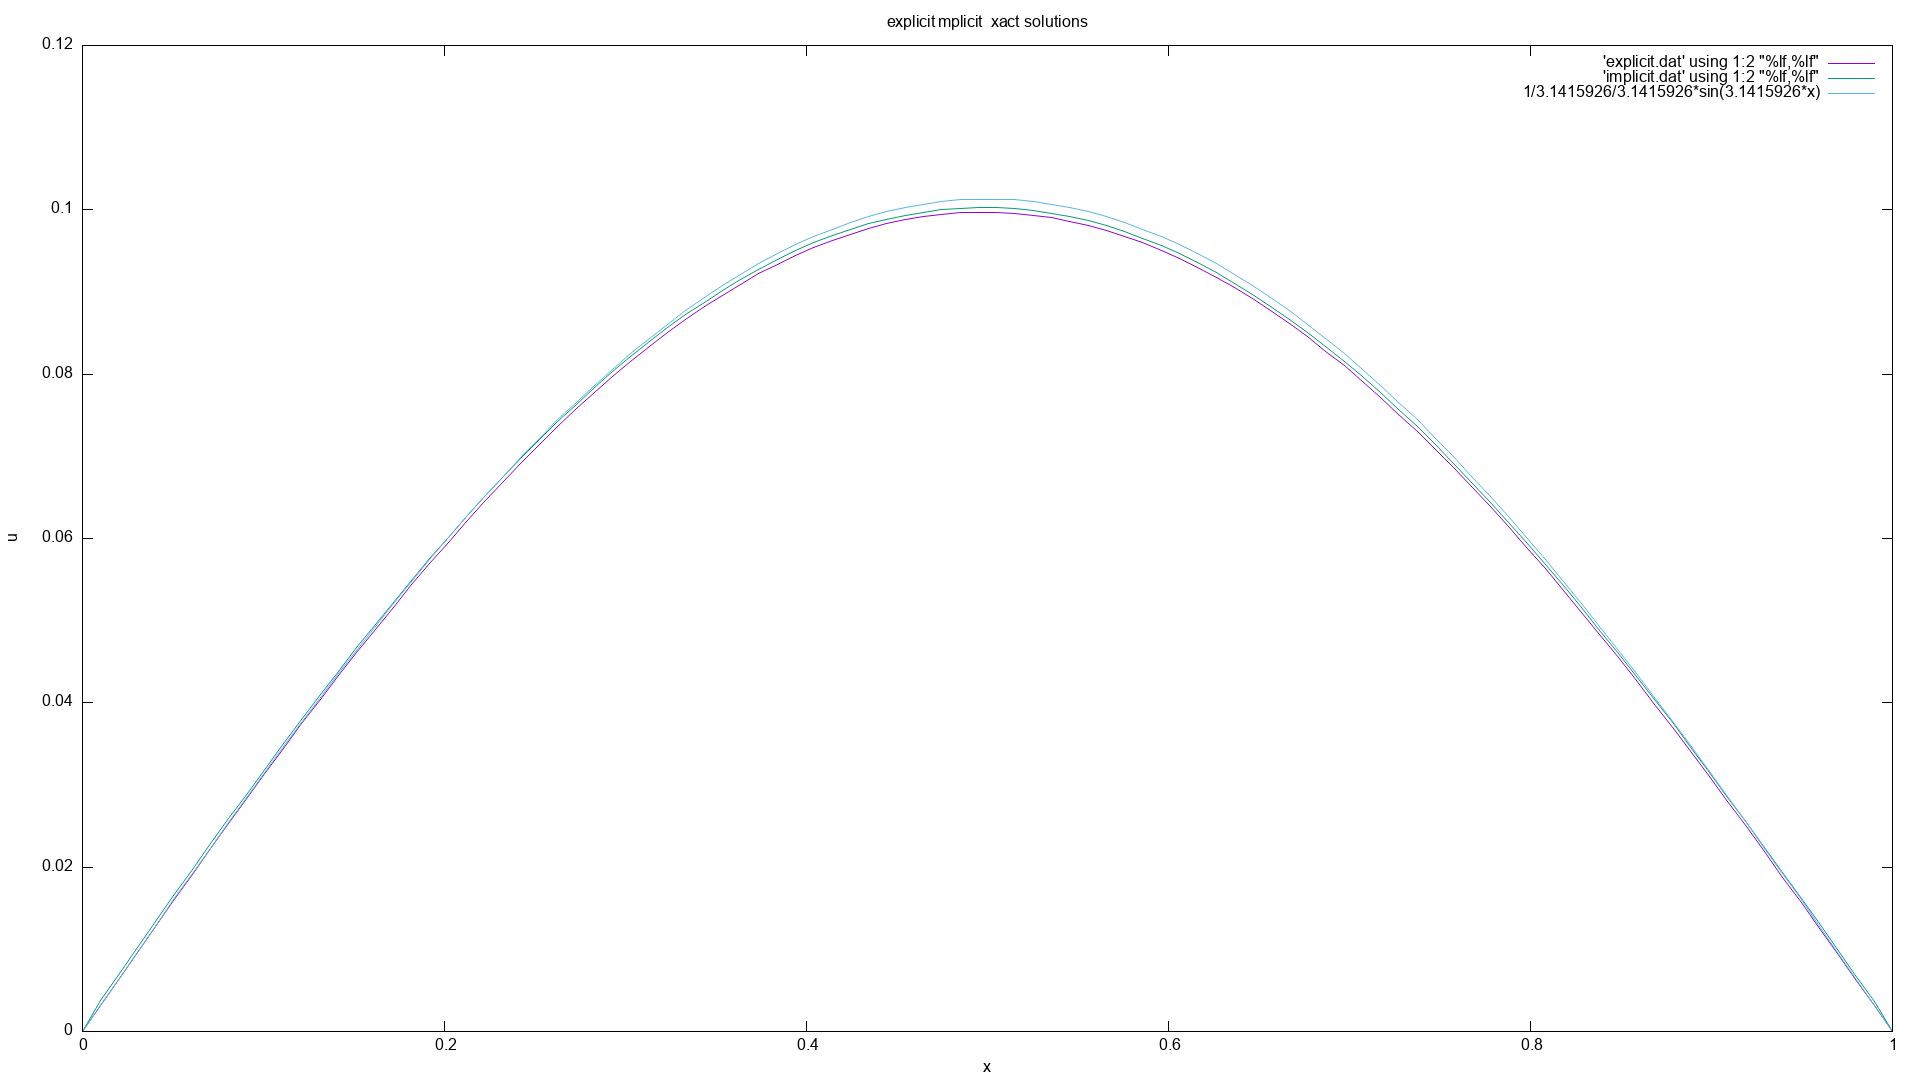
\includegraphics[scale=0.15]{./figures/solution_CFL0.2.png}
	\caption{solution CFL=0.2}
	\label{figure}
\end{figure}

\begin{figure}[htbp]
	\centering
	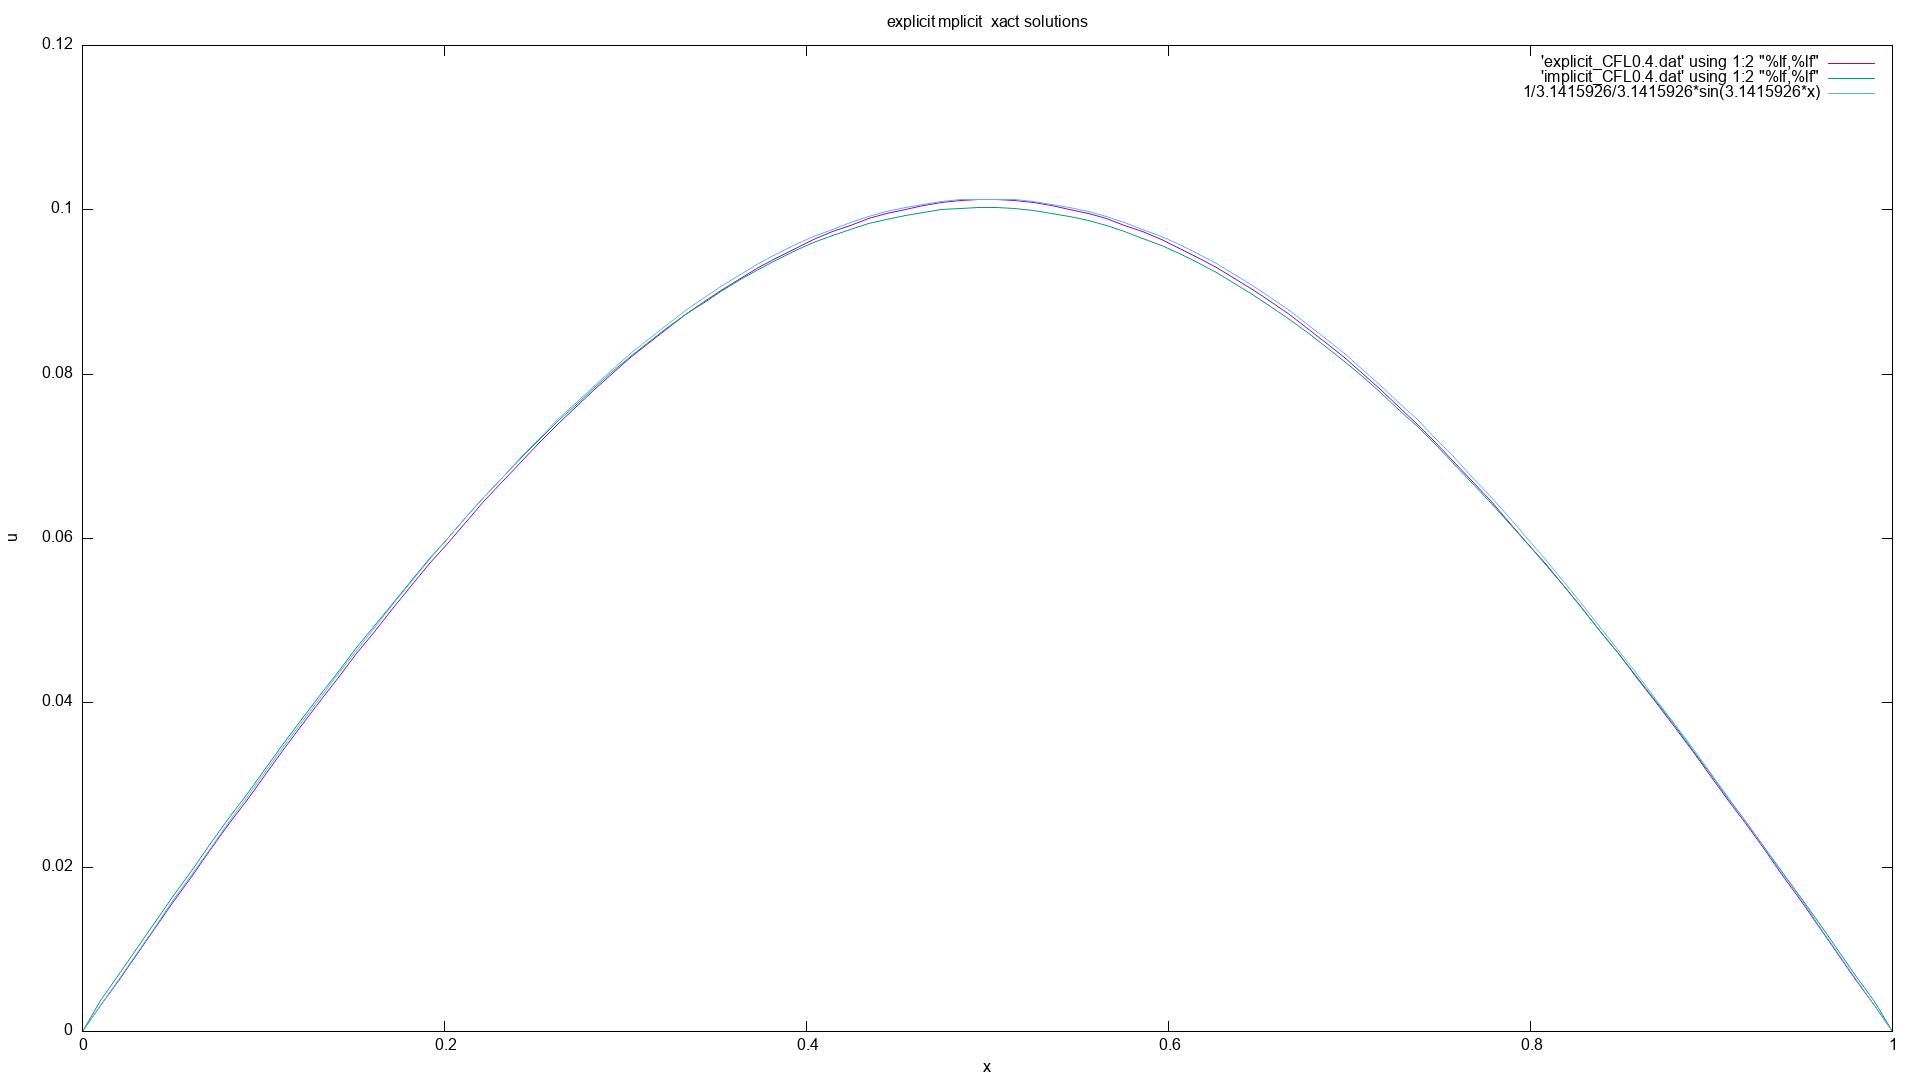
\includegraphics[scale=0.15]{./figures/solution_CFL0.4.png}
	\caption{solution CFL=0.4}
	\label{figure}
\end{figure}

%%%%%%%%%%%%%%%%%%%%%%%%%%%%%%%%%%%%%%%%%%%%%%%
\subsection{稳定性分析}
对于显式欧拉方法,根据公式(3)进行冯诺依曼稳定性分析,可以得到如下公式。
\begin{center}
	\begin{scriptsize}
		\begin{equation}
			\begin{aligned}
				\setlength{\abovedisplayskip}{-5pt}
				\delta u_{j}^{n+1}=\alpha * \delta u_{j-1}^{n}+(1-2 \alpha) * \delta u_{j}^{n}+\alpha * \delta u_{j+1}^{n} 
			\end{aligned}
		\end{equation}
	\end{scriptsize}
\end{center}
即有如下近似公式。
\begin{center}
	\begin{scriptsize}
		\begin{equation}
			\setlength{\abovedisplayskip}{-5pt}
\delta u_{j}^{n+1} \sim e^{\delta n \Delta t} * e^{i(k * j \Delta x)}
		\end{equation}
	\end{scriptsize}
\end{center}
\begin{center}
	\begin{scriptsize}
		\begin{equation}
			\begin{aligned}
				\setlength{\abovedisplayskip}{-5pt}
				e^{\delta \Delta t}&=\alpha * e^{i k \Delta x}+(1-2 * \alpha)+\alpha * e^{-i k \Delta x}\\
				&=\alpha *\left(e^{i k \Delta x}+e^{-i k \Delta x}\right)+(1-2 * \alpha) \\
				&=1-2 \alpha+2 \alpha \cos (k \Delta x)
			\end{aligned}
		\end{equation}
	\end{scriptsize}
\end{center}
根据稳定条件可以计算出$\alpha$的取值范围,在代码中用CFL表示$\alpha$。
\begin{center}
	\begin{scriptsize}
		\begin{equation}
			\begin{aligned}
			\setlength{\abovedisplayskip}{-5pt}
			|1-2 \alpha+2 \alpha \cos (k \Delta x)| \leq 1&\Rightarrow-1 \leq 1-4 \alpha \leq 1  \\
			&\Rightarrow 0 \leq \alpha \leq \frac{1}{2}
			\end{aligned}
		\end{equation}
	\end{scriptsize}
\end{center}
在3.1精度分析中,取$\alpha=0.2$,显式与隐式欧拉方法均稳定。

\begin{figure}[htbp]
	\centering
	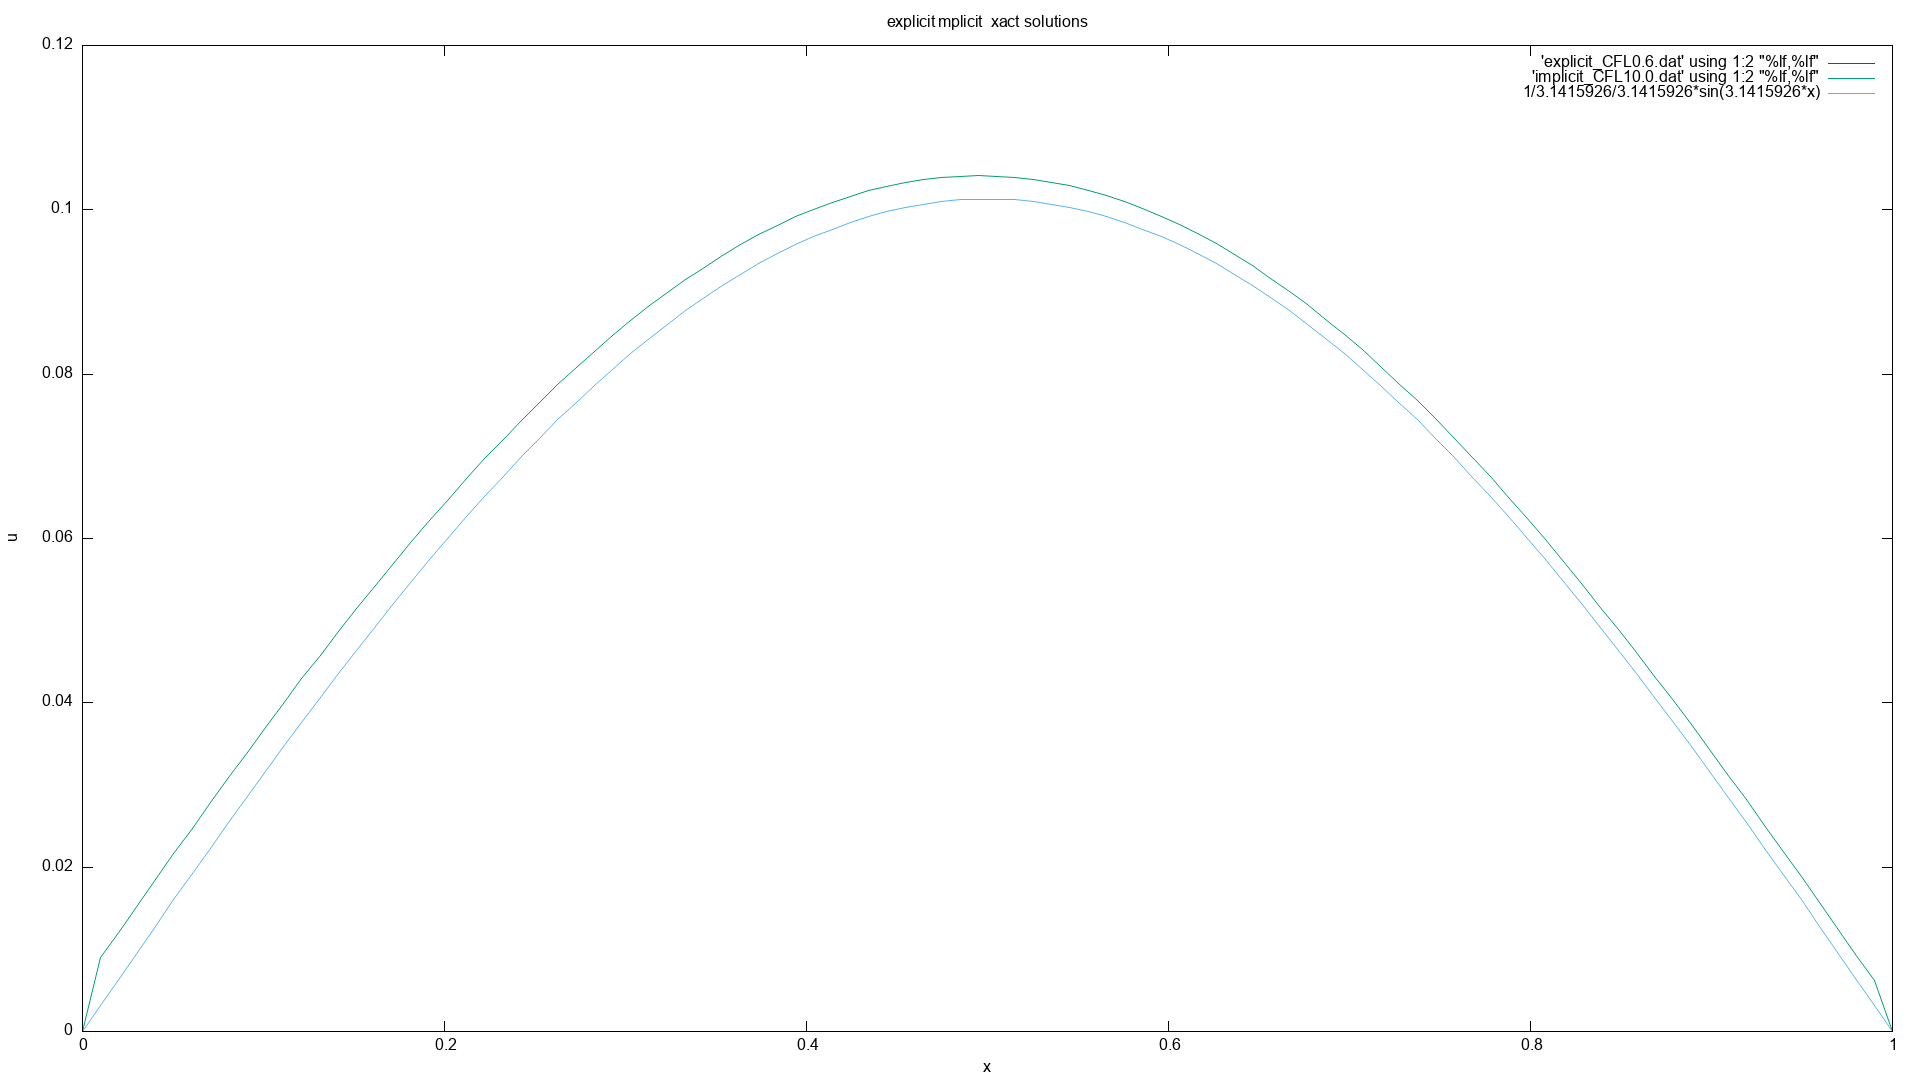
\includegraphics[scale=0.15]{./figures/solution_CFL_over05.png}
	\caption{solution CFL over 0.6}
	\label{figure}
\end{figure}

%%%%%%%%%%%%%%%%%%%%%%%%%%%%%%%%%%%%%%%%%%%%%%
\subsection{重启分析}

\subsection{并行分析}

\subsection{内存分析}


%%%%%%%%%%%%%%%%%%%%%%%%%%%%%%%%%%%%%%%%%%%%%%%%%%%%%%%%%%


\section{总结与展望}\label{sec:Conclusion}



\end{document}
